\section{Information Foraging}
Information Foraging Theory (IFT)~\cite{pirolli07} simplifies, in a principled way, analyzing information-seeking tasks by providing constructs borrowed from its optimal foraging theory roots. Optimal foraging theory describes predators that pursue prey through an environment, following scent from locality to locality. The predator is always trying to optimize their task. In IFT, the information seeker pursues information through an information environment. Scent, in the information environment, is a construct that exists in the forager's mind, representing their perception of where they might find information; this perception is shaped by proximal cues\textemdash hints provided by the information environment. Information foragers follow scent from locality to locality, information patch to information patch, pursuing their prey. 

Consider the following analogy: a forager is seeking berries. They go to a patch of berries, and estimate how many berries might be in that patch. They then pick berries until they decide that they have picked enough from this patch, and should move to the next one. In this model, proximal cues (how full the patch looks, how many berries nearby patches had), or scent, indicate to the forager how many berries might be in that patch. Of course, the forager might not estimate correctly how many berries there are if the indications are misleading, and they might switch to another patch too early (still easy berries to pick) or too late (time wasted looking for berries instead of switching patches). Building a correct estimate, and making berries easy to pick, so to speak, is an important application of IFT. 

The constructs provided by IFT were first used to analyze how a web user might search for information online~\cite{pirolliWeb}, modeling scent as relatedness of a link to the forager's prey. This work eventually developed into the WUFIS (Web User Flow by Information Scent) algorithm~\cite{wufis}. WUFIS represents network topology as a graph, where nodes are web pages and edges are the links that a user can click to navigate from one to another. IFT's scent is represented by relatedness of the words in a webpage to the forager's information need. The algorithm then predicts where the user will navigate by applying spreading activation. 

\begin{figure}
	\centering
	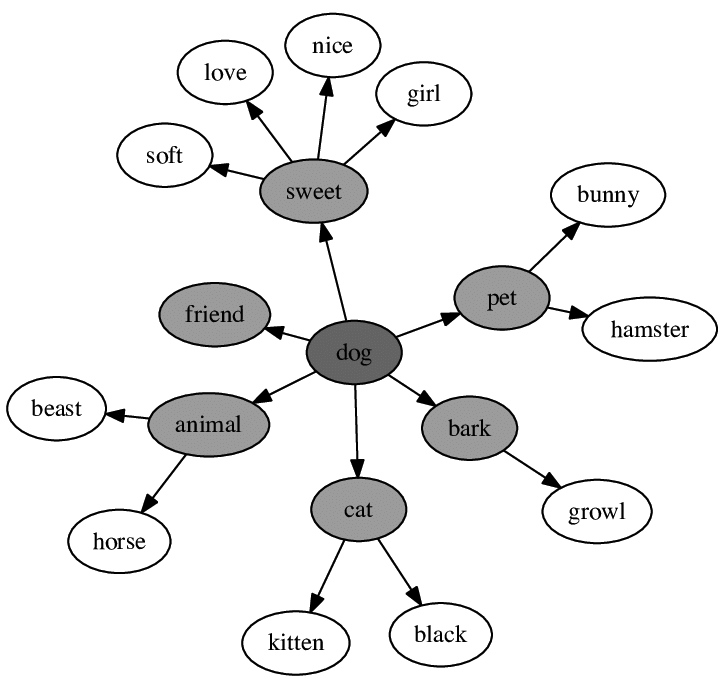
\includegraphics[width=0.5\linewidth]{spreading_example.png}
	\caption{Example of Spreading Activation in Neuroscience. ``Dog'' is initially activated; darker shading indicates higher activation. Source: ~\cite{spreadingexample}}
	\label{fig:activation}
\end{figure}

Spreading activation is a concept borrowed from neuroscience: Collins and Loftus ~\cite{spreadingactivation} posited that all memories and knowledge in our minds are connected in a network, and activating one memory also activates neighboring memories. Spreading activation, as adapted by the Information Foraging world, works by assigning one (or several) nodes in a graph with an initial activation of 1. Each edge in the graph is assigned with a weight. In the case of WUFIS, the weight is proportional to the similarity of the two nodes that the edge is connecting. In other cases, all edges are assigned the same weight. Each node in the graph is traversed, and the activation is ``spread'' to its children: typically, the parent node's activation is multiplied by the weight so that the child node's activation is lower. Each node, then, has an activaiton value that represents its similarity to the originally-activated node, as dictated by proximity to the original node and edge-weights. This mechanism can be seen in Figure \ref{fig:activation}. For WUFIS, spreading activation assigns each node with a value which represents the probability that a forager, given their current location and information need together with the scent of links connecting pages, will navigate to a specific page.

This spreading activation concept was utilized to model programmer navigation in the development of PFIS~\cite{pfis1a} and its subsequent revisions~\cite{pfis2,pfis3a}. PFIS built upon the spreading activation of WUFIS by applying it to the field of developer navigation~\cite{pfis1a}, inferring the forager's goal~\cite{pfis2}, and creating multi-factor models with PFIS~\cite{pfis3a}. In the programmer navigation domain, WUFIS web page nodes were now code fragments, and its edges were any click-able link that would navigate a developer from one fragment to another. When inferring the forager's goal, PFIS authors introduced the concept of heterogeneity to their network: in addition to linking code fragments, the PFIS algorithm also linked code fragments to key words (e.g., those extracted from a bug report), creating a more nuanced topology. Inspired by this heterogeneous approach, we take spreading activation to the socio-technical realm.

\section{Socio-Technical Networks}
In order to develop a spreading activation algorithm to answer requirements traceability questions in the socio-technical realm, we first examine work conducted in socio-technical graphs. Both Herbsleb and colleagues' socio-technical theory of coordination (STTC) ~\cite{herbsleb16}, and the Codebook project ~\cite{codebook} attempt to answer requirements traceability questions with socio-technical models. We begin by examining Herbsleb et al.'s work.

Herbsleb et al. conduct their work examining dependencies among engineering decisions\textemdash ``Who should work with whom?''. They answer this question by defining a constraint satisfaction problem that people must organize to solve. The theory draws from the key observation that the number of people was a powerful predictor of coordination problems (e.g., delay in development ~\cite{herbsleb03}), and quantifies people’s working relationships via a dependency network of work items. The solution to this problem provides an answer to the earlier ``Who should work with whom?'' question, which in turn serves as a unifying basis for solving a class of coordination problems, including expertise finding ~\cite{herbsleb02,herbsleb09}, cross-site communication ~\cite{herbsleb01}, and pull request acceptance in social coding environments ~\cite{herbsleb14}. While this STTC can address some of the traceability questions (e.g., ramifications ~\cite{ICSE30}), other questions that we want to answer, such as ``Which programmers are more error prone in their code according to the test results?'' ~\cite{lohar16}, need the relationships between people and artifacts. For a foundation that can answer all of our traceability questions, we turn to Codebook.

In the Codebook~\cite{codebook} project, people and work artifacts were ``friends'' in a social network. A user might be connected to an email they sent, bug they closed, and a commit they pushed; that commit has changes in code containing classes and calls. A sample Codebook topology can be seen in Figure \ref{fig:codebook}. By using a single data structure to represent these people, artifacts, and relationships, and a single algorithm (regular language reachability) to analyze this graph, Codebook could handle all the inter-team coordination problems identified in a survey responded by 110 Microsoft employees~\cite{codebook10}, including requirements traceability problems. 

\begin{figure}[ht!]
	\centering
	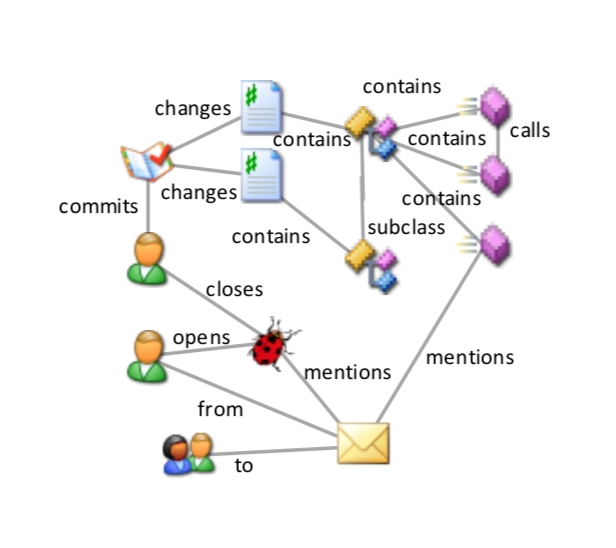
\includegraphics[width=0.5\linewidth]{codebook.png}
	\caption{The Codebook Topology, Source: ~\cite{codebook}}
	\label{fig:codebook}
\end{figure}

Codebook addresses problems by having a project personnel cast their coordination needs into regular expressions. For example, the requirements traceability question ``Which program manager wrote the specification for that code?'' could be addressed in Codebook with the regular expression ``\textsc{Code MentionedBy WordDocument AuthoredBy Person}''. This is a manual task, requiring a domain expert. In contrast, spreading activation can provide a mechanism for automated querying. We therefore adopt Codebook's underlying data structure, but instead of regular language reachability, we adapt the people-artifact graph for spreading activation.